\chapter{Implementazione e Test}

Questo capitolo tratta la descrizione della fase di implementazione e test della soluzione.
Ha l'obiettivo di documentare i passi effettuati per la costruzione della soluzione, e allo stesso tempo
si pone come guida al lettore, in caso volesse seguire il procedimento per poter creare una soluzione DLP.
\section{Predisposizione ambiente operativo}

L'ambiente di lavoro è così configurato:

\begin{itemize}
    \item Host: Macbook pro con MacOS BigSur v 11.2.3;
    \item Guest: Macchina virtuale con CentOS 8 installata su VirtualBox;
    \item Mail Server Postfix: installato su CentOS;
    \item Mail Client Outlook: installato sugli host della rete.
\end{itemize}

\subsection{Abilitare il port forwarding}
Per fare in modo che le macchine della rete locale possano avviare una connessione
verso il server (Postfix) viene utilizzata la modalità NAT di VirtualBox così da creare dei 
port-forwarding. È necessario dunque configurare la VM per l'utilizzo del NAT e aggiungere delle regole
per la traduzione della porta.
Le macchine si collegheranno all'indirizzo IP dell'Host utilizzando la porta Host Port configurata
per il forwarding e le connessioni verranno inoltrate da VirtualBox al Guest.
Per l'implementazione, la VM gestisce un mail server configurato per l'ascolto sulle porte 25, 465 e
587. Inoltre sono presenti anche altre due traduzioni, come mostrato nella tabella \ref{tabNAT}, per rendere raggiungibile un ipotetico web server e rendere possibile
la connessione SSH verso la macchina virtuale.

% Please add the following required packages to your document preamble:
% \usepackage{graphicx}
\begin{table}[htp]
    \centering
    \resizebox{\textwidth}{!}{%
    \begin{tabular}{|l|l|l|l|l|l|}
    \hline
    \textbf{Name} & \textbf{Protocol} & \textbf{Host IP} & \textbf{Host Port} & \textbf{Guest IP} & \textbf{Guest Port} \\ \hline
    http       & TCP &  & 8080 &  & 80  \\ \hline
    smtps      & TCP &  & 4444 &  & 465 \\ \hline
    smtp       & TCP &  & 2525 &  & 25  \\ \hline
    submission & TCP &  & 5555 &  & 587 \\ \hline
    ssh        & TCP &  & 2222 &  & 22  \\ \hline
    \end{tabular}%
    }
    \caption{Tabella di traduzione NAT di VirtualBox.}\label{tabNAT}
    \end{table}
\pagebreak
\subsection{Apertura porte del firewall}

Il secondo passo consiste nell’aprire le porte del firewall, necessarie per il funzionamento del progetto, 
in modo tale che le connessioni possano raggiungere il Guest. Questo è possibile attraverso i comandi:
\begin{verbatim}
    firewall-cmd --zone=public --permanent --add-port 587/tcp
    firewall-cmd --zone=public --permanent --add-port 465/tcp
    firewall-cmd --zone=public --permanent --add-port 25/tcp
    firewall-cmd --zone=public --permanent --add-port 80/tcp
    firewall-cmd --zone=public --permanent --add-port 22/tcp
\end{verbatim}
A questo punto è necessario effettuare un reload:

\begin{verbatim}
    firewall-cmd --reload
\end{verbatim}
Si può verificare che le porte siano state aperte correttamente attraverso il comando:
\begin{verbatim}
    firewall-cmd --list-all
\end{verbatim}
\begin{verbatim}
    [root@localhost palfag]# firewall-cmd --list-all
    public (active)
      target: default
      icmp-block-inversion: no
      interfaces: enp0s3
      sources: 
      services: cockpit dhcpv6-client ssh
      ports: 80/tcp 465/tcp 25/tcp 587/tcp 22/tcp
      protocols: 
      masquerade: no
      forward-ports: 
      source-ports: 
      icmp-blocks: 
      rich rules: 
\end{verbatim}
Nella voce \textit{ports:} sono listate tutte le porte correntemente aperte.
\pagebreak
\subsection{Prenotazione IP presso il server DHCP}
Un server DHCP ha il compito di assegnare ad un dispositivo che si connette alla sua rete il primo indirizzo IP 
valido disponibile. In generale ogni LAN possiede un server DHCP. 
Il compito principale è quello di assegnare a ciascun host che si connette alla LAN un indirizzo IP temporaneo, 
che sarà diverso tutte le volte che l’host si connette alla rete. 
%È possibile configurare DHCP in modo che un dato host riceva un indirizzo IP persistente, 
%ovvero che ogni volta che l’host entra nella rete, gli venga assegnato sempre lo stesso indirizzo IP. 
%Si procederà per quest’ultima via, in modo che l’indirizzo IP dell’host che ospita il mail server non cambi mai.

Poiché il server deve essere raggiungibile dalle macchine della rete, 
per il progetto si è deciso di specificare un indirizzo IP prenotato per l’host della LAN che ospiterà il mail server. 
Specificando un IP riservato, tale host riceverà sempre lo stesso indirizzo IP privato ogni volta che accede al 
server DHCP del router. In questo modo non sarà necessario modificare le impostazioni dei mail client, 
installati sulle altre macchine, ogni volta che il server cambia IP.
Per la prenotazione di un indirizzo IP si dovrà accedere nella pagina di configurazione del router, 
accessibile attraverso il browser, digitando l’indirizzo IP del router nella barra di ricerca 
(in questo caso 192.168.8.1). Fatto ciò, si dovrà accedere alle impostazioni avanzate e cliccare sulla voce DHCP. 
A questo punto sarà necessario inserire una riga di traduzione, come mostrato nella tabella \ref{reserveIPtable},
associando il MAC (indirizzo di livello 2) del dispositivo interessato, all’indirizzo IP che si vuole che ottenga 
ogni volta che ne richieda uno al server DHCP.

\begin{table}[htp]
    \centering
    \resizebox{\textwidth}{!}{%
    \begin{tabular}{|l|l|l|l|l|}
    \hline
    \rowcolor[HTML]{EFEFEF} 
    \textbf{N.} & \textbf{Indirizzo IP} & \textbf{Nome Dispositivo} & \textbf{MAC}      & \textbf{Opzioni}          \\ \hline
    1           & 192.168.8.150         & Macbook-di-Paolo              & 9A:0A:05:52:3F:07 & \multicolumn{1}{c|}{canc} \\ \hline
    \end{tabular}%
    }
    \caption{Tabella per l'assegnazione di un indirizzo IP riservato}\label{reserveIPtable}
    \end{table}

\subsection{Generazione certificato per l'utilizzo del protocollo TLS/SSL}
Per poter utilizzare il protocollo TLS/SSL è necessario generare un certificato\cite{certs}.
Si può generare il certificato attraverso il comando:

\begin{verbatim}
    sudo openssl req -x509 -nodes -days 365 -newkey rsa:2048 
        -keyout /etc/pki/tls/private/apache-selfsigned.key 
        -out /etc/pki/tls/certs/apache-selfsigned.crt
\end{verbatim}

\begin{itemize}
    \item \textit{openssl}: questo è il comando che serve per generare il certificato e la chiave;
    \item \textit{req -x509}: specifica che si desidera utilizzare la gestione della richiesta di firma del certificato 
    (CSR) X.509. X.509 è uno standard di infrastruttura a chiave pubblica a cui aderiscono SSL e TLS per la gestione 
    di chiavi e certificati;
    \item \textit{-nodes}: questa opzione dice a OpenSSL di saltare il passo per inserire una password di protezione al certificato;
    \item \textit{-days 365}: questa opzione imposta la durata del certificato, ovvero quanto tempo sarà considerato
    valido;
    \item \textit{-newkey rsa:2048}: questa opzione specifica la creazione di una chiave assieme al certificato, 
    utilizzata per firmarlo. La chiave è generata attraverso il cifrario asimmetrico RSA 
    e possiede una lunghezza pari a 2048 bit.
    \item \textit{-keyout}: questa opzione specifica dove andare a posizionare all’interno del 
    file system la chiave privata che verrà creata.
    \item \textit{-out}: questa opzione specifica dove andare a posizionare all’interno del file system il certificato che verrà creato.
\end{itemize}
A questo punto è necessario inserire una serie di informazioni, a scopo progettuale sono stati compilati soltanto:

\begin{verbatim}
    Country Name (2 letter code) [XX]:IT
    Common Name (your server's hostname) []: mail.palfag.it
\end{verbatim}
e verrà creato il seguente certificato:

\begin{verbatim}
    -----BEGIN CERTIFICATE-----
    MIIDLTCCAhWgAwIBAgIUcO18m3JGVMQusLW4i3+AHqrZjDkwDQYJKoZIhvcNAQEL
    BQAwJjELMAkGA1UEBhMCaXQxFzAVBgNVBAMMDm1haWwucGFsZmFnLml0MB4XDTIx
    MDQyNzA5MDUxMVoXDTIyMDQyNzA5MDUxMVowJjELMAkGA1UEBhMCaXQxFzAVBgNV
    BAMMDm1haWwucGFsZmFnLml0MIIBIjANBgkqhkiG9w0BAQEFAAOCAQ8AMIIBCgKC
    AQEAo0JQF4b1t6aXcMxnzda8kb8ILbXh3DosjA/GsuJl2DQcsXiPB6pGxcvx/NoZ
    q7jVmXWYh5U/VAfjnWjziculuzKMg941NrzsR9lZzBb9ts323o/rWEnDpDtu9fYo
    nB/egn/VGPx0bwSC90sMXcIop96n7/aWU7cCUXmx2iDCNSXeM5RUVD0B+zILTLoq
    D5T8O304Zyq/3okHm52nAqhLCaMz3OI4eIcI3rnUBMl/Qah5h4QzN2KcD6lAMsQv
    bdNz71nw0KGtj6w7b7E5GriIuTfzH+TTJvsHZercAxeOknAbUVnYuJOwB9TTsriQ
    g03kM6c9bsDqtDP4IiDbZOq7fwIDAQABo1MwUTAdBgNVHQ4EFgQUspg7MbB/qLaH
    S+7PIo2dmZU2znowHwYDVR0jBBgwFoAUspg7MbB/qLaHS+7PIo2dmZU2znowDwYD
    VR0TAQH/BAUwAwEB/zANBgkqhkiG9w0BAQsFAAOCAQEAoYsSvmJMP/o750iHyn60
    W4InLhNMszCdh2wGKZXDpQEK+WLSIVzBYnByr5EHmRQLs9RcXMbArKF2NyW+QADv
    1lBkUwa3CZidEkLUKlbqYaBJu1j2k/RsIAGrRBiy40rOr0JjHrRfpJBx1NafjkA+
    Y/zSk6Z7Th5xgCcYVPx+dOtljCtGJ0fGrwdrGpywSKzV6OkbPtDQz9rppk17aKRW
    tb5l1Kyrq5RMq7dvSOTxtveglpceHduMAusU98fBb6zBIhbujkLfbyDY6fUTLsJB
    L43NSn6EzXghKY/KPViYkAjiBlpTNjkBhRrwfqYBJoyi4RyOgwu26HaX8EcTe9yv
    aQ==
    -----END CERTIFICATE-----
\end{verbatim}
È necessario tenere a mente dove sono stati posizionati, all’interno del file system, 
certificato e chiave privata poiché sono necessari, in una fase successiva, per la configurazione di Postfix.

\section{Installazione e configurazione di Postfix}

\begin{figure}[htp]
    \centering
    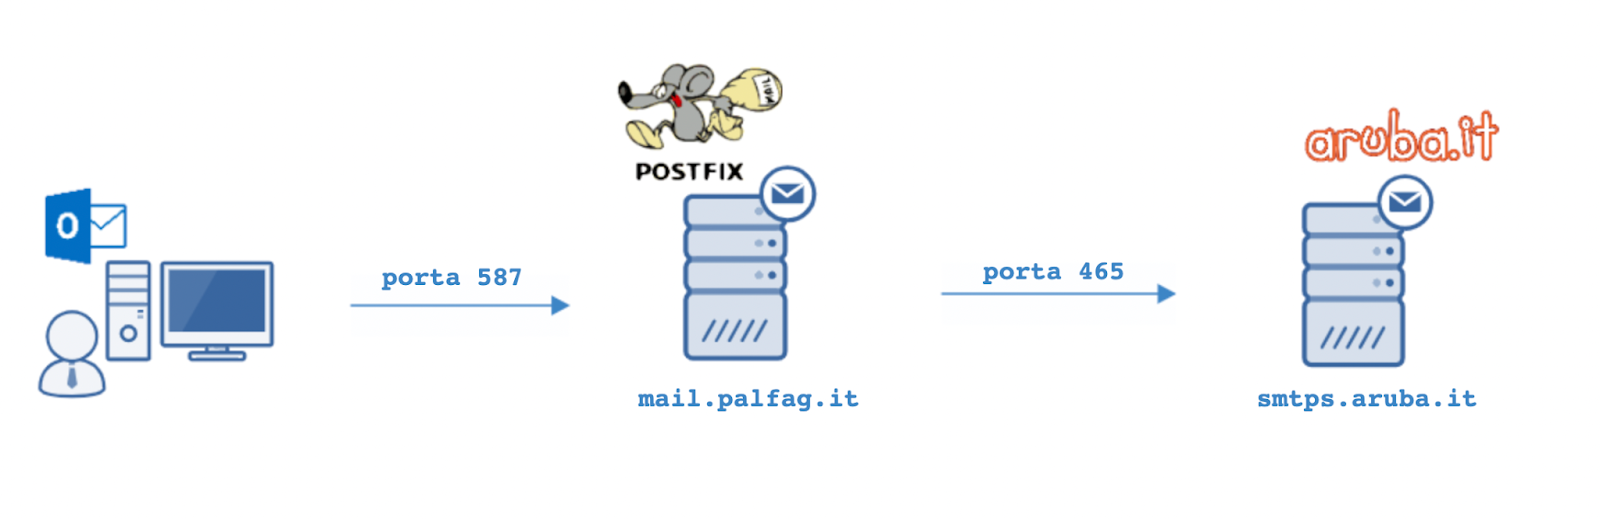
\includegraphics[width=12cm, height=20cm, keepaspectratio]{Screenshot 2021-05-03 at 11.28.07.png}
    \caption{Configurazione di Postfix}\label{confPostfix}
  \end{figure}
La figura \ref{confPostfix} mostra le varie componenti che prendono parte alla configurazione e le relative porte
utilizzate per lo scambio dei messaggi di posta.
\newline
\newline
1. Innanzitutto è necessario installare i seguenti pacchetti:

\begin{verbatim}
    yum install postfix mailx cyrus-sasl cyrus-sasl-plain
\end{verbatim}
2. Creare un file, in questo caso è stato chiamato \textit{sasl\_passwd} dove saranno inserite le credenziali
necessarie per l'autenticazione presso il server Aruba:

\begin{verbatim}
    nano /etc/postfix/sasl_passwd
    [smtps.aruba.it]:465    paolo.fagioli@certimeter.it:pwd
\end{verbatim}
3. Processare il file contenente le credenziali:

\begin{verbatim}
    postmap /etc/postfix/sasl_passwd
\end{verbatim}
4. Editare il file \textit{/etc/postfix/main.cf}:

\begin{verbatim}
    myhostname = mail.palfag.it
    relayhost= [smtps.aruba.it]:465
    mynetworks = 192.168.8.0/24 127.0.0.0/8
    smpd_banner = $myhostname ESMTP $mail_name ($mail_version)
    mailbox_size_limit = 0
    inet_interfaces = all
    inet_protocols = all
    append_dot_mydomain = no
    readme_directory = no
\end{verbatim}
5. Sempre all'interno del file \textit{/etc/postfix/main.cf} inserire i parametri per la configurazione di TLS,
in questo momento sono necessari il certificato e la chiave precedentemente generati:

\begin{verbatim}
    # TLS parameters
    smtpd_tls_cert_file=/etc/pki/tls/certs/apache-selfsigned.crt
    smtpd_tls_key_file=/etc/pki/tls/private/apache-selfsigned.key

    smtpd_tls_security_level=encrypt
    smtp_tls_CApath=/etc/ssl/certs
    smtp_tls_security_level=encrypt
    smtp_tls_session_cache_database = btree:${data_directory}/smtp_scache
    smtp_sasl_password_maps = hash:/etc/postfix/sasl_passwd
    smtp_tls_wrappermode = yes
    smtp_use_tls = yes
    smtp_sasl_auth_enable = yes
    smtp_sasl_security_options = noanonymous
\end{verbatim}
6. Avviare Postfix:
\begin{verbatim}
    systemctl start postfix.service
\end{verbatim}
7. A questo punto è possibile verificare il corretto funzionamento della funzione di inoltro verso i server di Aruba 
provando ad inviare una email da terminale:

\begin{verbatim}
    echo corpo | mail -s “Oggetto” -r emailMittente emailDestinatario 
\end{verbatim}
8. Una volta testato il funzionamento, è necessario configurare Postfix in modo che ascolti dalle porte 465 e 587 
(la porta 25 è già configurata di default).

Editare il file \textit{/etc/postfix/master.cf}. Attraverso la seguente configurazione Postfix ascolterà 
sulla porta 587 e sarà dotato di tutte le impostazioni necessarie per supportare il protocollo TLS:

\begin{verbatim}
    submission inet n       -       n       -       -       smtpd
  -o syslog_name=postfix/submission
  -o smtpd_sasl_auth_enable=yes
  -o smtpd_sasl_security_options=noanonymous
  -o broken_sasl_auth_clients=yes
  -o smtpd_tls_security_level=encrypt
  -o smtpd_tls_key_file=/etc/pki/tls/private/apache-selfsigned.key
  -o smtpd_tls_cert_file=/etc/pki/tls/certs/apache-selfsigned.crt
  -o smtpd_tls_loglevel=1
  -o smtpd_tls_session_cache_timeout=3600s
  -o smtpd_tls_session_cache_database=btree:/var/lib/postfix/smtpd_tls_cache
  -o tls_random_source=dev:/dev/urandom
  -o tls_random_exchange_name=/var/lib/postfix/prng_exch
  -o smtpd_tls_auth_only=yes
  -o smtpd_recipient_restrictions=permit_sasl_authenticated,reject
  -o smtpd_relay_restrictions=permit_sasl_authenticated,reject
\end{verbatim}
9. Un procedimento simile per fare in modo che ascolti anche dalla porta 465:

\begin{verbatim}
    smtps     inet  n       -       n       -       -       smtpd
    -o syslog_name=postfix/smtps
    -o smtpd_sasl_auth_enable=yes
    -o smtpd_sasl_security_options=noanonymous
    -o broken_sasl_auth_clients=yes
    -o smtpd_recipient_restrictions=permit_sasl_authenticated,reject
    -o smtpd_tls_security_level=encryptà
    -o smtpd_tls_wrappermode=yes
    -o smtpd_tls_key_file=/etc/pki/tls/private/apache-selfsigned.key
    -o smtpd_tls_cert_file=/etc/pki/tls/certs/apache-selfsigned.crt
    -o smtpd_tls_loglevel=1
    -o smtpd_tls_session_cache_timeout=3600s
    -o smtpd_tls_session_cache_database=btree:/var/lib/postfix/smtpd_tls_cache
    -o tls_random_source=dev:/dev/urandom
    -o tls_random_exchange_name=/var/lib/postfix/prng_exch
    -o smtpd_tls_auth_only=yes
\end{verbatim}
10. Avviare sasl\_authd
\begin{verbatim}
    systemctl start sasl_authd.services
\end{verbatim}
11. Riavviare Postfix
\begin{verbatim}
    systemctl restart postfix.service
\end{verbatim}

Da questo momento Postfix è pronto per svolgere il suo lavoro.

\section{Configurazione Microsoft Outlook}
Il client di posta elettronica standard utilizzato in azienda è Microsoft Outlook, 
per questo motivo la configurazione avverrà con quest'ultimo, 
ma ovviamente il procedimento è analogo utilizzando client mail diversi come ad esempio Mozilla Thunderbird.
Per configurare il client di posta MS Outlook è necessario avviare il software.
A questo punto andare su ``File'' e fare click su ``Aggiungi account''.

Nella finestra proposta inserire il proprio indirizzo di posta aziendale e selezionare ``Consenti la configurazione
manuale dell'account'' e poi fare click su ``Connetti''.

Nella schermata successiva selezionare la voce ``IMAP'' e compilare i campi come mostrato nella tabella \ref{serverOUT}.


\begin{table}[htp]
    \centering
    \begin{tabular}{|l|l|l|}
    \hline
    \rowcolor[HTML]{EFEFEF} 
    \textbf{Posta in arrivo} & imaps.aruba.it & 993  \\ \hline
    \textbf{Posta in uscita} & mail.palfag.it & 5555 \\ \hline
    \end{tabular}%
    \caption{Configurazione server in entrata e in uscita}\label{serverOUT}
    \end{table}
    Si ricorda che la porta 5555 inserita è una porta effimera che successivamente verrà tradotta nella porta 587
    dal NAT di VirtualBox.
    Selezionare la spunta ``Usa SSL per connetterti'', a questo punto dovremmo trovarci nella stessa situazione
    della figura \ref{confOutlook}.

        \begin{figure}[htp]
            \centering
            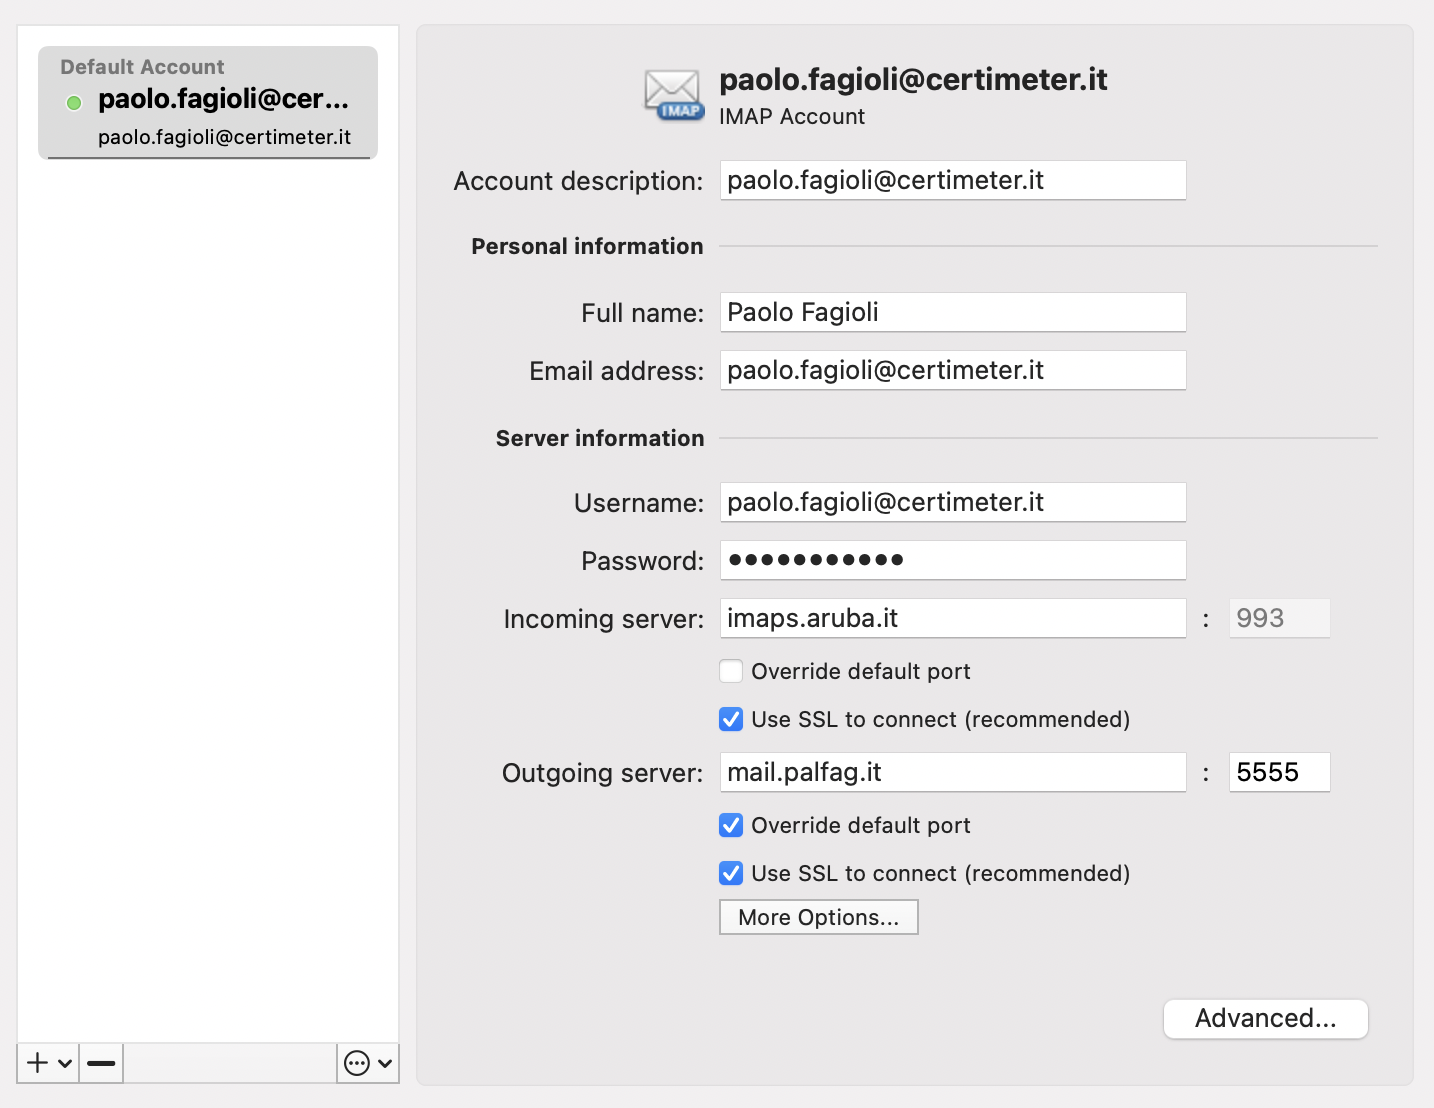
\includegraphics[width=12cm, height=20cm, keepaspectratio]{confOutlook.png}
            \caption{Configurazione di Outlook}\label{confOutlook}
        \end{figure}   
        
        \begin{figure}[htp]
          \centering
          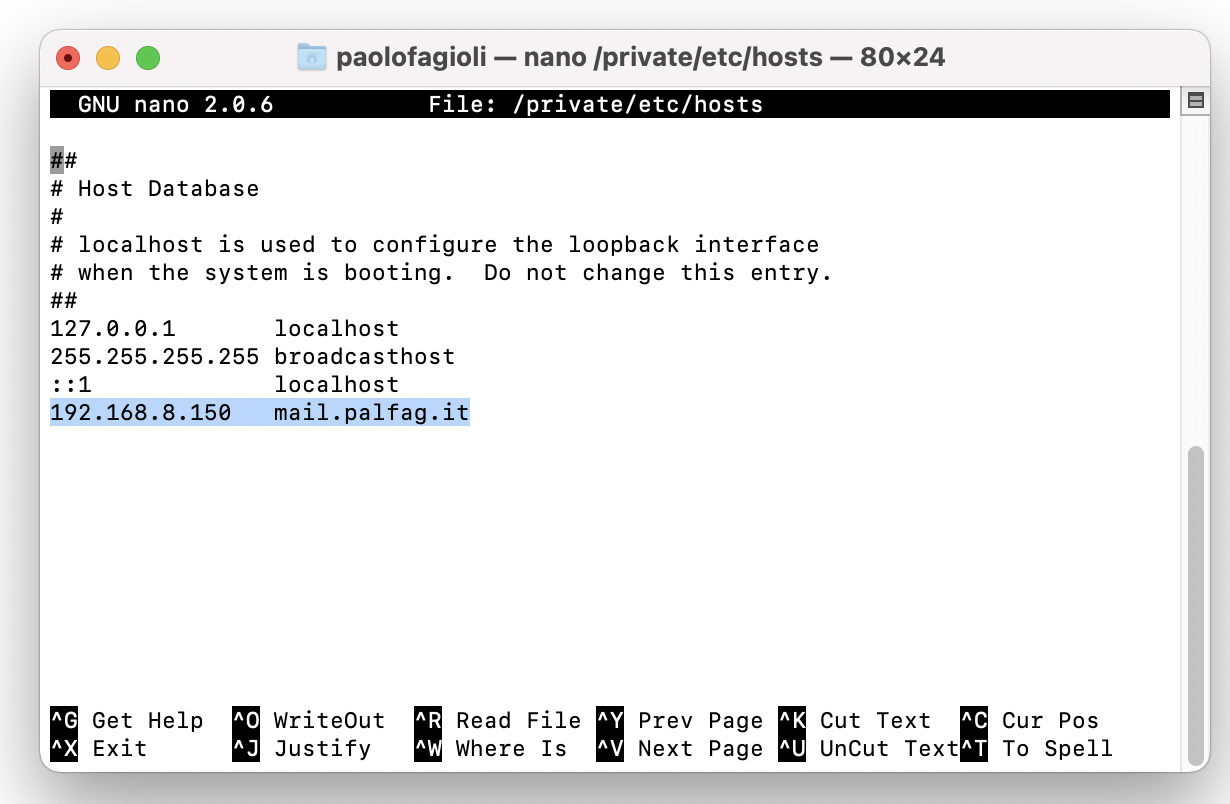
\includegraphics[width=12cm, height=20cm, keepaspectratio]{hosts.png}
          \caption{Aggiunta record di traduzione DNS.}\label{hosts}
      \end{figure}  
    Poiché il dominio mail.palfag.it non è registrato, 
    nessun server DNS sarebbe in grado di compiere la traduzione in 192.168.8.150, 
    è dunque necessario inserire un record di traduzione manualmente all’interno del file \textit{/private/etc/hosts} 
    come mostrato nella figura \ref{hosts}.

    
    In realtà in azienda ci sarà un server DNS con il compito di tradurre il dominio in indirizzo IP, 
    e quindi, non sarebbe necessario modificare il file \textit{/private/etc/hosts} su ogni macchina aziendale.


    A questo punto è già possibile testare il funzionamento provando ad inviare una email attraverso Outlook. 
    Dovrebbe spuntare un avviso dicendo che il certificato è autofirmato e quindi non attendibile. 
    È necessario istruire il nostro computer a fidarsi sempre del certificato
    (anche in questo caso in azienda non ci sarebbe bisogno di effettuare questo passaggio, poiché 
    il certificato non sarebbe autofirmato, ma firmato da una certificate authority).

    Una volta fatto questo, risulta possibile inviare le email con Outlook.


    \section{Architettura finale}
    Una volta effettuate tutte le configurazioni necessarie, è possibile migliorare il disegno dell’architettura. 
    Il disegno risultante è mostrato in figura \ref{archFinal}.

    \begin{figure}[htp]
        \centering
        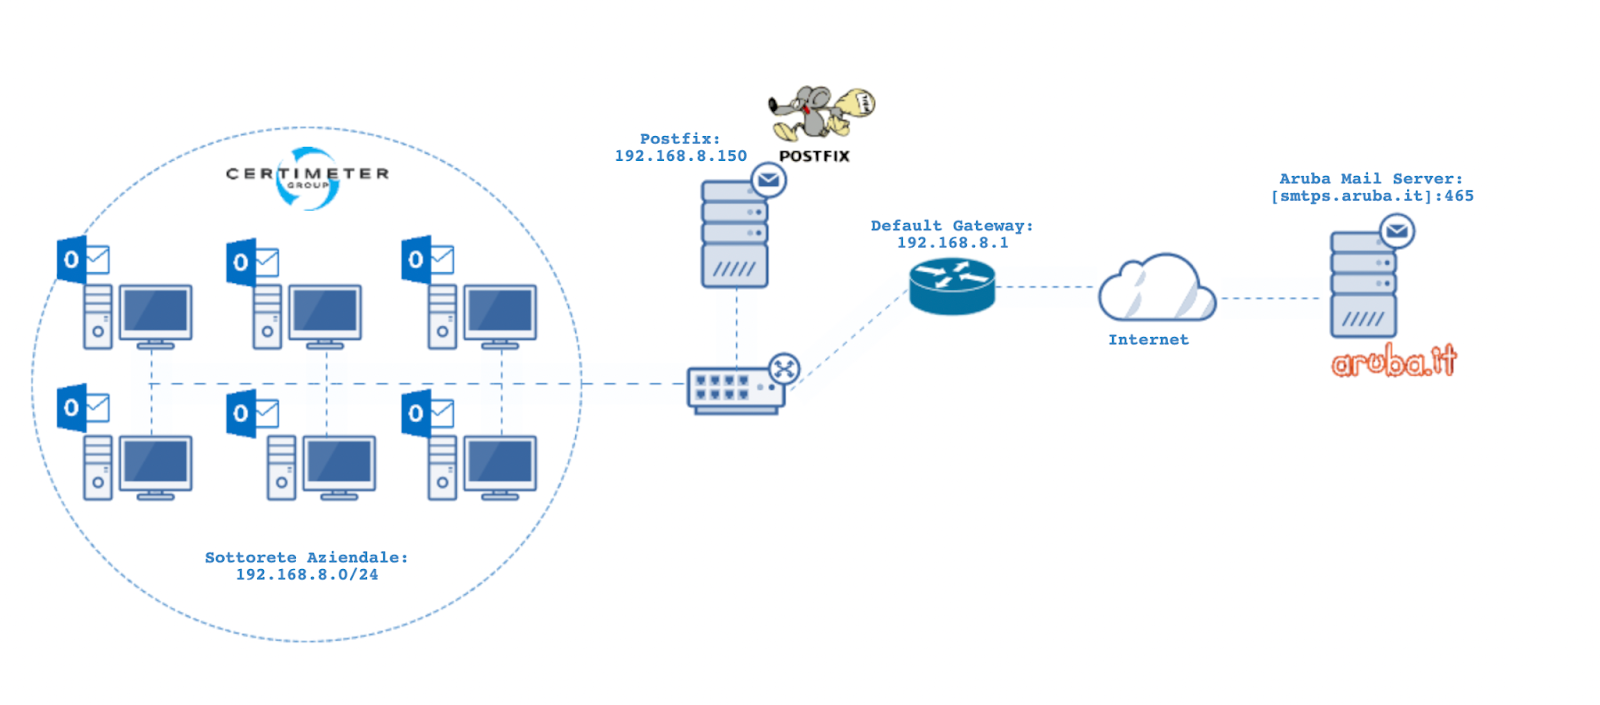
\includegraphics[width=12cm, height=20cm, keepaspectratio]{arch_final.png}
        \caption{Architettura finale.}\label{archFinal}
    \end{figure} 

    Tutti i Mail User Agent sono configurati in modo da avere come server SMTP di uscita mail.palfag.it, 
    per la traduzione del dominio, ogni host della rete contatterà il server DNS aziendale, il cui compito è
    quello di risolvere il dominio mail.palfag.it -> 192.168.8.150.

    All'invio di una email da parte di un dipendente, questa verrà indirizzata a Postfix (192.168.8.150) che la 
    ispezionerà. Nel caso in cui dovesse bloccare l’invio della email per via del contenuto riservato, 
    Postfix provvederà ad avvisare il mittente del suo rifiuto di consegnare il messaggio.

    Nel caso in cui il messaggio sia autorizzato ad essere inoltrato, Postfix attiverà la sua funzione di inoltro 
    girandolo verso i mail server di Aruba. Fisicamente consegnerà il frame al suo default gateway.

    %\pagebreak
    \section{Configurazione di controlli interni}
    Per lo sviluppo di filtri è necessario come prima cosa, se non esistono, creare i file:

    \begin{itemize}
        \item header\_checks
        \item mime\_header\_checks
        \item body\_checks
    \end{itemize}

    All'interno del file header\_checks sono definiti dei controlli per il filtraggio degli header
    (From:, To:, Subject:, ecc\dots), body\_checks definisce i controlli sul corpo del messaggio e
    infine mime\_header\_checks sugli allegati. È importante notare che il controllo degli allegati
    nativo di Postfix permette soltanto di filtrare in base al nome del file e all'estensione. 
    Nei paragrafi successivi è definito un filtro esterno per l'analisi del contenuto degli allegati.

    Una volta creati i file, è necessario aggiungere al file \textit{/etc/postfix/main.cf} le seguenti tre righe:

    \begin{verbatim}
        header_checks = regexp:/etc/postfix/header_checks
        mime_header_checks = regexp:/etc/postfix/mime_header_checks
        body_checks = regexp:/etc/postfix/body_checks
    \end{verbatim}

    Postfix utilizza questi file per effettuare il filtraggio dei contenuti (es. corpo e oggetto) e anche del
    contesto (es. mittente e destinatario). Sono definiti più file perché Postfix permette di utilizzare regole 
    diverse per filtrare cose diverse, ad esempio oggetto e corpo del messaggio.

    \section{Sviluppo di filtri interni}
    In questa sezione viene documentato lo sviluppo di una serie di filtri per fare in modo che Postfix possa 
    rilevare eventuali email da bloccare così da prevenire eventuali fuoriuscite dal sistema aziendale di dati riservati. 
    Vengono utilizzate le espressioni regolari per lo sviluppo dei filtri. Per ogni filtro sviluppato è possibile 
    decidere in che modo si vuole che reagisca Postfix al verificarsi dell’evento, 
    ovvero quando rileva in un’email un contenuto identificato riservato, oppure quando riceve un’email da un 
    mittente inserito in una blacklist.
    I controlli hanno la seguente struttura: “se si verifica questo, allora fai quello”, 
    infatti nella prima parte viene inserito il pattern del contenuto da rilevare, mentre nella seconda viene 
    specificata l’azione di risposta da intraprendere.

    I filtri sviluppati si dividono in due macro-aree:

    \begin{enumerate}
        \item Analisi del contenuto;
        \item Analisi del contesto.
    \end{enumerate}

    \subsection{Analisi del contenuto}
    Questo tipo di controlli si occupa del filtraggio del contenuto dell'email, 
    andando a ispezionare oggetto, corpo del messaggio ed eventuali allegati. 
    
    Sono utilizzate le espressioni regolari per individuare e bloccare messaggi di posta che contengono dati
    finanziari (ad esempio Carte VISA), o per permetterne l’invio eliminando il contenuto riservato. 
    
    Importante ricordare che Postfix effettua il controllo riga per riga, quindi se viene identificato un 
    contenuto riservato, e come azione di risposta si scegliesse IGNORE, 
    l’intera riga sarà eliminata (questo potrebbe compromettere l’integrità/significato originale del messaggio). 
    
    Sono inseriti dei controlli sull’oggetto utilizzando parole chiave che, se presenti, 
    porteranno al blocco dell’invio o alla quarantena del messaggio. Per gli allegati invece è possibile, nativamente,
    effettuare controlli esclusivamente sul filename o sull’estensione. 

    \subsubsection{Controlli sull'oggetto (file header\_checks):}

    1. Blocco delle email che contengono le parole chiave: URGENTE, TOP SECRET, SENSIBILE, SEGRETO.
    In questo caso Postfix bloccherà il messaggio e avviserà il mittente della decisione intrapresa.

    \begin{verbatim}
    /^Subject:(.)*(URGENTE | TOP SECRET| … | SEGRETO)(.)*/
        REJECT Il server ha bloccato il messaggio per 
        la possibile presenza di dati sensibili
    \end{verbatim}
    2. Quarantena dei messaggi che contengono la parola chiave PRIVATO:
    \begin{verbatim}
    /^Subject:(.)*PRIVATO(.)*/
        HOLD Il server ha messo in quarantena il messaggio per 
        la possibile presenza di dati sensibili
    \end{verbatim}
    3. Blocco dei messaggi che hanno come oggetto una carta VISA:
    \begin{verbatim}
    /^Subject:(.)*([0-9]{4}( |-)*){3}[0-9]{4}(.)*/
        REJECT EMAIL BLOCCATA: CARTA VISA RICONOSCIUTA
    \end{verbatim}


    \subsubsection{Controlli sull'allegato (file mime\_header\_checks):}

    1. Blocco delle email che contengono allegati con estensione .ZIP:

    \begin{verbatim}
    /^(.)*name=\"(.*)\.zip\"/
        REJECT allegato ZIP Bloccato
    \end{verbatim}

    \subsubsection{Controlli sul corpo (file body\_checks):}

    1. Blocco carte VISA presenti nel corpo del messaggio:
    \begin{verbatim}
    /^(.)*([0-9]{4}( |-)*){3}[0-9]{4}(.)*/
        REJECT EMAIL BLOCCATA: CARTA VISA RICONOSCIUTA
    \end{verbatim}
    2. Eliminazione del codice fiscale presente nel messaggio:
    \begin{verbatim}
    /^(.)*([A-z]){6}([0-9]){2}[A-z]([0-9]){2}[A-z][0-9]{3}[A-z](.)*/
        IGNORE CODICE FISCALE RIMOSSO DAL MESSAGGIO
    \end{verbatim}


    \subsection{Analisi del contesto}
    I controlli che si occupano di analizzare il contesto vanno a esaminare le restanti 
    informazioni che compongono l’email. Sono stati creati, ad esempio, controlli per filtrare in base al 
    mittente del messaggio o del destinatario e controlli che bloccano i messaggi inviati verso uno specifico dominio.
    % e si può scegliere che Postfix 
    %non accetti email che provengono da un account di posta elettronica diverso da quello aziendale 
    %(nome.cognome@certimeter.it). 

    \subsubsection{Mettere in blacklist un mittente:}
    Come impostazione di default Postfix accetta le email che provengono da qualunque indirizzo di posta, 
    tuttavia è possibile inserire un mittente in blacklist in modo che Postfix rifiuti tutte le email che 
    provengono dal suo indirizzo di posta. Vi sono diverse possibilità per mettere un mittente in blacklist, 
    tuttavia tutte effettuano un controllo sull’header FROM: del messaggio.

    \begin{verbatim}
    /^From:(.)*francesco.lorusso@certimeter.it(.)*/
        REJECT  SENDER ADDRESS REJECTED: BLACKLISTED
    \end{verbatim}

    \subsubsection{Blocco delle email indirizzate verso il dominio topolino.it:}
    Si suppone che da policy aziendali sia vietato, per i dipendenti, 
    inviare email al dominio topolino.it.
    In questo caso viene inserito il seguente filtro:

    \begin{verbatim}
    /^To:.*@topolino.it/
        REJECT RECIPIENT DOMAIN BANNED
    \end{verbatim}

    %\subsubsection{Blocco delle email inviate da caselle di posta differenti da quelle aziendali:}
    %\begin{verbatim}
    %if /^From:/
    %!/(^From:.*@certimeter.it)/ 
    %    REJECT SENDER NON-CORPORATE DOMAIN REJECTED
    %endif
    %\end{verbatim}

    \section{Script Python esterno per la gestione degli allegati}
    Il filtraggio dei contenuti di Postfix è abbastanza limitato, poiché non permette di analizzare il contenuto
    degli allegati. Postfix però prevede la possibilità di utilizzare dei plug-in esterni. Per questo motivo è stato
    sviluppato uno script Python che permettesse l'analisi e l'identificazione di contenuti riservati presenti 
    negli allegati.


    \section{Shell code}
    Nel suo sito ufficiale Postfix offre uno script bash di esempio \cite{Postfix3}, che è stato personalizzato per 
    permettere il dialogo tra il mail server e lo script sviluppato in Python.
    In ingresso lo script \textit{wrapper.sh} riceve il file .eml da Postfix, che gira allo script Python,  
    il cui compito è quello di analizzare il contenuto degli allegati.
    lo script \textit{wrapper.sh} avrà comportamenti differenti a seconda del valore restituito dallo script Python:
    
    
    \begin{enumerate}
        \item se sys.exit(0): ritorna l' email a Postfix in modo che possa continuare il percorso;
        \item se sys.exit(1): il messaggio viene rifiutato poiché identificati dati riservati. 
        (Postfix invia una email di ritorno al mittente spiegando perché ha dovuto bloccare il messaggio). 
    \end{enumerate}

    \begin{verbatim}
1 #!/bin/sh
2 
3 # Simple shell-based filter. It is meant to be invoked as follows:
4 #       /path/to/script -f sender recipients...
5 
6 # Localize these. The -G option does nothing before Postfix 2.3.
7 INSPECT_DIR=/var/spool/filter
8 SENDMAIL="/usr/sbin/sendmail -G -i" # NEVER NEVER NEVER use "-t" here.
9 
10 # Exit codes from <sysexits.h>
11 EX_TEMPFAIL=75
12 EX_UNAVAILABLE=69
13 
14 # Clean up when done or when aborting.
15 trap "rm -f in.$$" 0 1 2 3 15
16 
17 # Start processing.
18 cd $INSPECT_DIR || {
19     echo $INSPECT_DIR does not exist; exit $EX_TEMPFAIL; }
20 
21 cat >in.$$ || { 
22     echo Cannot save mail to file; exit $EX_TEMPFAIL; }
23 
24 # Specify your content filter here.
25 # python3 /media/shared/my_filter.py <in.$$ || {
26 #   echo Message content rejected; exit $EX_UNAVAILABLE; }
27 
28 $SENDMAIL "$@" <in.$$
29 
30 exit $?
    \end{verbatim}

    \section{Integrazione script esterno}
    Per fare in modo che venga eseguito il filtro esterno, è necessario configurare Postfix in modo
    che consegni l'email allo script.
    \newline
    \newline
    1. Prima di tutto si deve aggiungere al file \textit{/etc/postfix/master.cf} il filtro:

    \begin{verbatim}
    /etc/postfix/master.cf:
    # =============================================================
    # service type  private unpriv  chroot  wakeup  maxproc command
    #               (yes)   (yes)   (yes)   (never) (100)
    # =============================================================
    my_filter unix	  -	      n	      n	      -	      -	    pipe
	    flags=Rq user=filter 
        argv=/home/filter/wrapper.sh -f ${sender} -- ${recipient}
    \end{verbatim}
    In questo modo è stato registrato il filtro chiamato ``my\_filter''.
    \newline
    \newline
    2. Poi bisogna dire a Postfix di eseguire lo script quando riceve le email sulla porta 587 (submission):

    \begin{verbatim}
        /etc/postfix/master.cf:
    # =============================================================
    # service type  private unpriv  chroot  wakeup  maxproc command
    #               (yes)   (yes)   (yes)   (never) (100)
    # =============================================================
    submission inet   n       -       n        -      -      smtpd
            -o content_filter=my_filter:  
    \end{verbatim}
    3. Infine si deve riavviare Postfix:

    \begin{verbatim}
    postfix reload 
    \end{verbatim}
    
\pagebreak
    \section{Test}
    In questo paragrafo sono documentati i test effettuati volti a collaudare la soluzione DLP 
    implementata e a verificarne il corretto funzionamento.

    \subsection{Test sull'analisi del contenuto}


\begin{table}[htp]
    \centering
    \resizebox{\textwidth}{!}{%
    \begin{tabular}{ll}
    \multicolumn{2}{c}{test 1 (TS01): \textbf{Messaggio contenente parola chiave da bloccare}}                                                              \\ \hline
    \rowcolor[HTML]{EFEFEF} 
    \multicolumn{1}{|l|}{\cellcolor[HTML]{EFEFEF}ID}    & \multicolumn{1}{l|}{\cellcolor[HTML]{EFEFEF}TS01}                            \\ \hline
    \multicolumn{1}{|l|}{Nome}                          & \multicolumn{1}{l|}{Messaggio contenente parola chiave}                      \\ \hline
    \rowcolor[HTML]{EFEFEF} 
    \multicolumn{1}{|l|}{\cellcolor[HTML]{EFEFEF}Descrizione} &
      \multicolumn{1}{l|}{\cellcolor[HTML]{EFEFEF}\begin{tabular}[c]{@{}l@{}}il messaggio inviato contiene la parola chiave \\ TOP SECRET come oggetto del messaggio\end{tabular}} \\ \hline
    \multicolumn{1}{|l|}{\begin{tabular}[c]{@{}l@{}}Messaggio inviato\\ dal mittente\end{tabular}} &
      \multicolumn{1}{l|}{\begin{tabular}[c]{@{}l@{}}Subject: Top secret\\ From: Paolo Fagioli <paolo.fagioli@certimeter.it>\\ To: Paolo Fagioli <palfag33@gmail.com>\\ \\ Test TS01\end{tabular}} \\ \hline
    \rowcolor[HTML]{EFEFEF} 
    \multicolumn{1}{|l|}{\cellcolor[HTML]{EFEFEF}Risultato atteso} &
      \multicolumn{1}{l|}{\cellcolor[HTML]{EFEFEF}\begin{tabular}[c]{@{}l@{}}Verrà attivata la clausola REJECT, il messaggio\\ sarà rifiutato da Postfix e verrà avvisato il \\ mittente.\end{tabular}} \\ \hline
    \multicolumn{1}{|l|}{Risultato ottenuto} &
      \multicolumn{1}{l|}{\begin{tabular}[c]{@{}l@{}}Postfix ha rifiutato il messaggio. Il mittente ha \\ ricevuto il seguente avviso:\\ \\ Il server ha bloccato il messaggio per\\ la possibile presenza di dati sensibili.\end{tabular}} \\ \hline
    \rowcolor[HTML]{EFEFEF} 
    \multicolumn{1}{|l|}{\cellcolor[HTML]{EFEFEF}Esito} & \multicolumn{1}{l|}{\cellcolor[HTML]{EFEFEF}{\color[HTML]{333333} SUPERATO}} \\ \hline
    \end{tabular}%
    }
    \end{table}


\begin{table}[htp]
    \centering
    \resizebox{\textwidth}{!}{%
    \begin{tabular}{ll}
    \multicolumn{2}{c}{test 2 (TS02): \textbf{Messaggio privo di dati sensibili}} \\ \hline
    \rowcolor[HTML]{EFEFEF} 
    \multicolumn{1}{|l|}{\cellcolor[HTML]{EFEFEF}ID} &
      \multicolumn{1}{l|}{\cellcolor[HTML]{EFEFEF}TS02} \\ \hline
    \multicolumn{1}{|l|}{Nome} &
      \multicolumn{1}{l|}{Messaggio privo di dati sensibili} \\ \hline
    \rowcolor[HTML]{EFEFEF} 
    \multicolumn{1}{|l|}{\cellcolor[HTML]{EFEFEF}Descrizione} &
      \multicolumn{1}{l|}{\cellcolor[HTML]{EFEFEF}\begin{tabular}[c]{@{}l@{}}il messaggio inviato non contiene alcun dato\\ riservato\end{tabular}} \\ \hline
    \multicolumn{1}{|l|}{\begin{tabular}[c]{@{}l@{}}Messaggio inviato\\ dal mittente\end{tabular}} &
      \multicolumn{1}{l|}{\begin{tabular}[c]{@{}l@{}}Subject: Benvenuto!\\ From: Paolo Fagioli <paolo.fagioli@certimeter.it>\\ To: Paolo Fagioli <palfag33@gmail.com>\\ \\ \\ Ciao Paolo,\\ Benvenuto nel Team <3\end{tabular}} \\ \hline
    \rowcolor[HTML]{EFEFEF} 
    \multicolumn{1}{|l|}{\cellcolor[HTML]{EFEFEF}Risultato atteso} &
      \multicolumn{1}{l|}{\cellcolor[HTML]{EFEFEF}\begin{tabular}[c]{@{}l@{}}In questo caso Postfix si comporterà da normale\\ mail server di inoltro. Il messaggio verrà \\ inoltrato presso i mail server di Aruba.\end{tabular}} \\ \hline
    \multicolumn{1}{|l|}{Risultato ottenuto} &
      \multicolumn{1}{l|}{\begin{tabular}[c]{@{}l@{}}Come da previsione il messaggio è stato\\ inoltrato correttamente. Il destinatario ha \\ ricevuto il seguente messaggio:\\ \\ Subject: Benvenuto!\\ From: Paolo Fagioli <paolo.fagioli@certimeter.it>\\ To: Paolo Fagioli <palfag33@gmail.com>\\ \\ Ciao Paolo,\\ Benvenuto nel Team <3\end{tabular}} \\ \hline
    \rowcolor[HTML]{EFEFEF} 
    \multicolumn{1}{|l|}{\cellcolor[HTML]{EFEFEF}Esito} &
      \multicolumn{1}{l|}{\cellcolor[HTML]{EFEFEF}{\color[HTML]{333333} SUPERATO}} \\ \hline
    \end{tabular}%
    }
    \end{table}

\begin{table}[htp]
    \centering
    \resizebox{\textwidth}{!}{%
    \begin{tabular}{ll}
    \multicolumn{2}{c}{test 3 (TS03): \textbf{Messaggio contenente dati personali}}                                                                                   \\ \hline
    \rowcolor[HTML]{EFEFEF} 
    \multicolumn{1}{|l|}{\cellcolor[HTML]{EFEFEF}ID}          & \multicolumn{1}{l|}{\cellcolor[HTML]{EFEFEF}TS03}                                            \\ \hline
    \multicolumn{1}{|l|}{Nome}                                & \multicolumn{1}{l|}{Messaggio contenente dati personali}                                     \\ \hline
    \rowcolor[HTML]{EFEFEF} 
    \multicolumn{1}{|l|}{\cellcolor[HTML]{EFEFEF}Descrizione} & \multicolumn{1}{l|}{\cellcolor[HTML]{EFEFEF}il messaggio inviato contiene un codice fiscale} \\ \hline
    \multicolumn{1}{|l|}{\begin{tabular}[c]{@{}l@{}}Messaggio inviato\\ dal mittente\end{tabular}} &
      \multicolumn{1}{l|}{\begin{tabular}[c]{@{}l@{}}Subject: Aggiornamento\\ From: Paolo Fagioli <paolo.fagioli@certimeter.it>\\ To: Paolo Fagioli <palfag33@gmail.com>\\ \\ Salve invio quanto richiesto,\\ Nominativo:\\ 	Paolo Fagioli\\ Codice fiscale:\\ 	TCMDPW34L46D127O\\ Buona giornata,\\ Paolo\end{tabular}} \\ \hline
    \rowcolor[HTML]{EFEFEF} 
    \multicolumn{1}{|l|}{\cellcolor[HTML]{EFEFEF}Risultato atteso} &
      \multicolumn{1}{l|}{\cellcolor[HTML]{EFEFEF}\begin{tabular}[c]{@{}l@{}}Verrà attivata la clausola IGNORE, il codice\\ fiscale sarà rimosso e la restante parte del\\ messaggio verrà ricevuta dal destinatario.\end{tabular}} \\ \hline
    \multicolumn{1}{|l|}{Risultato ottenuto} &
      \multicolumn{1}{l|}{\begin{tabular}[c]{@{}l@{}}Postfix si è comportato come previsto, eliminando\\ il codice fiscale dal messaggio. Il messaggio\\ ricevuto dal destinatario è il seguente:\\ \\ Salve invio quanto richiesto,\\ Nominativo:\\         Paolo Fagioli\\ Codice fiscale:\\ \\ Buona giornata,\\ Paolo\end{tabular}} \\ \hline
    \rowcolor[HTML]{EFEFEF} 
    \multicolumn{1}{|l|}{\cellcolor[HTML]{EFEFEF}Esito}       & \multicolumn{1}{l|}{\cellcolor[HTML]{EFEFEF}SUPERATO}                                        \\ \hline
    \end{tabular}%
    }
    \end{table}


\begin{table}[htp]
    \centering
    \resizebox{\textwidth}{!}{%
    \begin{tabular}{ll}
    \multicolumn{2}{c}{test 4 (TS04): \textbf{Messaggio contenente dati finanziari}} \\ \hline
    \rowcolor[HTML]{EFEFEF} 
    \multicolumn{1}{|l|}{\cellcolor[HTML]{EFEFEF}ID} &
      \multicolumn{1}{l|}{\cellcolor[HTML]{EFEFEF}TS04} \\ \hline
    \multicolumn{1}{|l|}{Nome} &
      \multicolumn{1}{l|}{Messaggio contenente dati finanziari} \\ \hline
    \rowcolor[HTML]{EFEFEF} 
    \multicolumn{1}{|l|}{\cellcolor[HTML]{EFEFEF}Descrizione} &
      \multicolumn{1}{l|}{\cellcolor[HTML]{EFEFEF}\begin{tabular}[c]{@{}l@{}}il messaggio inviato contiene il numero di una\\ carta di pagamento VISA\end{tabular}} \\ \hline
    \multicolumn{1}{|l|}{\begin{tabular}[c]{@{}l@{}}Messaggio inviato\\ dal mittente\end{tabular}} &
      \multicolumn{1}{l|}{\begin{tabular}[c]{@{}l@{}}Subject: pagamento\\ From: Paolo Fagioli <paolo.fagioli@certimeter.it>\\ To: Paolo Fagioli <palfag33@gmail.com>\\ \\ Ciao,\\ ti invio il numero della carta:\\ 4839-9268-2312-5203\\ Mi raccomando usala solo per urgenze.\\ Paolo\end{tabular}} \\ \hline
    \rowcolor[HTML]{EFEFEF} 
    \multicolumn{1}{|l|}{\cellcolor[HTML]{EFEFEF}Risultato atteso} &
      \multicolumn{1}{l|}{\cellcolor[HTML]{EFEFEF}\begin{tabular}[c]{@{}l@{}}Verrà attivata la clausola REJECT, il messaggio\\ sarà rifiutato da Postfix e verrà avvisato il\\ mittente.\end{tabular}} \\ \hline
    \multicolumn{1}{|l|}{Risultato ottenuto} &
      \multicolumn{1}{l|}{\begin{tabular}[c]{@{}l@{}}Postfix ha rifiutato il messaggio. Il mittente ha\\ ricevuto il seguente avviso:\\ \\ EMAIL BLOCCATA: \\ CARTA VISA RICONOSCIUTA\end{tabular}} \\ \hline
    \rowcolor[HTML]{EFEFEF} 
    \multicolumn{1}{|l|}{\cellcolor[HTML]{EFEFEF}Esito} &
      \multicolumn{1}{l|}{\cellcolor[HTML]{EFEFEF}{\color[HTML]{333333} SUPERATO}} \\ \hline
    \end{tabular}%
    }
    \end{table}

    \pagebreak

\begin{table}[htp]
    \centering
    \resizebox{\textwidth}{!}{%
    \begin{tabular}{ll}
    \multicolumn{2}{c}{test 5 (TS05): \textbf{Messaggio contenente allegato riservato}}                                                         \\ \hline
    \rowcolor[HTML]{EFEFEF} 
    \multicolumn{1}{|l|}{\cellcolor[HTML]{EFEFEF}ID}    & \multicolumn{1}{l|}{\cellcolor[HTML]{EFEFEF}TS05}                            \\ \hline
    \multicolumn{1}{|l|}{Nome}                          & \multicolumn{1}{l|}{Messaggio contenente allegato riservato}                 \\ \hline
    \rowcolor[HTML]{EFEFEF} 
    \multicolumn{1}{|l|}{\cellcolor[HTML]{EFEFEF}Descrizione} &
      \multicolumn{1}{l|}{\cellcolor[HTML]{EFEFEF}\begin{tabular}[c]{@{}l@{}}il messaggio inviato contiene come allegato.\end{tabular}} \\ \hline
    \multicolumn{1}{|l|}{\begin{tabular}[c]{@{}l@{}}Messaggio inviato\\ dal mittente\end{tabular}} &
      \multicolumn{1}{l|}{\begin{tabular}[c]{@{}l@{}}Subject: test\\ From: Paolo Fagioli <paolo.fagioli@certimeter.it>\\ To: Paolo Fagioli <palfag33@gmail.com>\\ \\ test con allegato.\end{tabular}} \\ \hline
    \rowcolor[HTML]{EFEFEF} 
    \multicolumn{1}{|l|}{\cellcolor[HTML]{EFEFEF}Risultato atteso} &
      \multicolumn{1}{l|}{\cellcolor[HTML]{EFEFEF}\begin{tabular}[c]{@{}l@{}}Il filtro nativo di Postfix non troverà nulla, passerà\\ il messaggio al filtro esterno sviluppato in Python.\\ Il filtro esterno troverà il contenuto riservato e \\ bloccherà l'invio, e verrà inviata una email di \\ rimbalzo al mittente.\end{tabular}} \\ \hline
    \multicolumn{1}{|l|}{Risultato ottenuto} &
      \multicolumn{1}{l|}{\begin{tabular}[c]{@{}l@{}}Il risultato ottenuto conferma le aspettative.\\ Il mittente riceve la seguente email:\\ \\ Subject: Undelivered Mail Returned to Sender\\ From: Mail Delivery System <MAILER-DAEMON@mail.palfag.it>\\ To: Paolo Fagioli <paolo.fagioli@certimeter.it>\\ \\ Message content rejected\end{tabular}} \\ \hline
    \rowcolor[HTML]{EFEFEF} 
    \multicolumn{1}{|l|}{\cellcolor[HTML]{EFEFEF}Esito} & \multicolumn{1}{l|}{\cellcolor[HTML]{EFEFEF}{\color[HTML]{333333} SUPERATO}} \\ \hline
    \end{tabular}%
    }
    \end{table}

    \begin{figure}[!b]
        \centering
        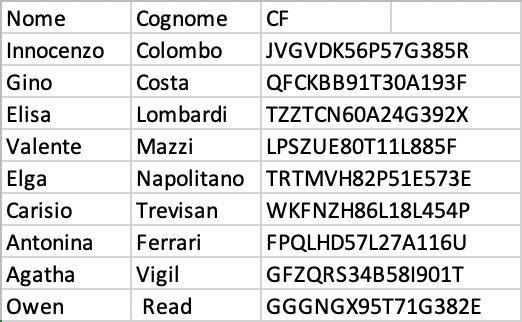
\includegraphics[width=8cm, height=10cm, keepaspectratio]{allegato_excel.png}
        \caption{Allegato elenco\_dipendenti.csv}\label{allegatoExcel}
      \end{figure}

    

    %\pagebreak

\begin{table}[htp]
    \centering
    \resizebox{\textwidth}{!}{%
    \begin{tabular}{ll}
    \multicolumn{2}{c}{test 6 (TS06): \textbf{Messaggio contenente allegato innocuo}} \\ \hline
    \rowcolor[HTML]{EFEFEF} 
    \multicolumn{1}{|l|}{\cellcolor[HTML]{EFEFEF}ID} &
      \multicolumn{1}{l|}{\cellcolor[HTML]{EFEFEF}TS06} \\ \hline
    \multicolumn{1}{|l|}{Nome} &
      \multicolumn{1}{l|}{Messaggio contenente allegato innocuo} \\ \hline
    \rowcolor[HTML]{EFEFEF} 
    \multicolumn{1}{|l|}{\cellcolor[HTML]{EFEFEF}Descrizione} &
      \multicolumn{1}{l|}{\cellcolor[HTML]{EFEFEF}\begin{tabular}[c]{@{}l@{}}il messaggio inviato contiene come allegato\\ un file word non contenente dati sensibili.\\ \\ allegato: poesia.doc\end{tabular}} \\ \hline
    \multicolumn{1}{|l|}{\begin{tabular}[c]{@{}l@{}}Messaggio inviato\\ dal mittente\end{tabular}} &
      \multicolumn{1}{l|}{\begin{tabular}[c]{@{}l@{}}Subject: test\\ From: Paolo Fagioli <paolo.fagioli@certimeter.it>\\ To: Paolo Fagioli <palfag33@gmail.com>\\ \\ test con allegato.\end{tabular}} \\ \hline
    \rowcolor[HTML]{EFEFEF} 
    \multicolumn{1}{|l|}{\cellcolor[HTML]{EFEFEF}Risultato atteso} &
      \multicolumn{1}{l|}{\cellcolor[HTML]{EFEFEF}\begin{tabular}[c]{@{}l@{}}Il filtro nativo di Postfix non troverà nulla, passerà\\ il messaggio al filtro esterno sviluppato in Python.\\ Il filtro esterno non troverà alcun contenuto riservato e \\ restituirà l'email a Postfix tramite il comando sendmail.\\ L'email sarà inoltrata ai mail server di Aruba.\end{tabular}} \\ \hline
    \multicolumn{1}{|l|}{Risultato ottenuto} &
      \multicolumn{1}{l|}{\begin{tabular}[c]{@{}l@{}}Il risultato ottenuto conferma le aspettative.\\ Il mittente ha ricevuto l'email originale contenente il file word.\end{tabular}} \\ \hline
    \rowcolor[HTML]{EFEFEF} 
    \multicolumn{1}{|l|}{\cellcolor[HTML]{EFEFEF}Esito} &
      \multicolumn{1}{l|}{\cellcolor[HTML]{EFEFEF}{\color[HTML]{333333} SUPERATO}} \\ \hline
    \end{tabular}%
    }
    \end{table}

    \begin{figure}[htp]
        \centering
        \fbox{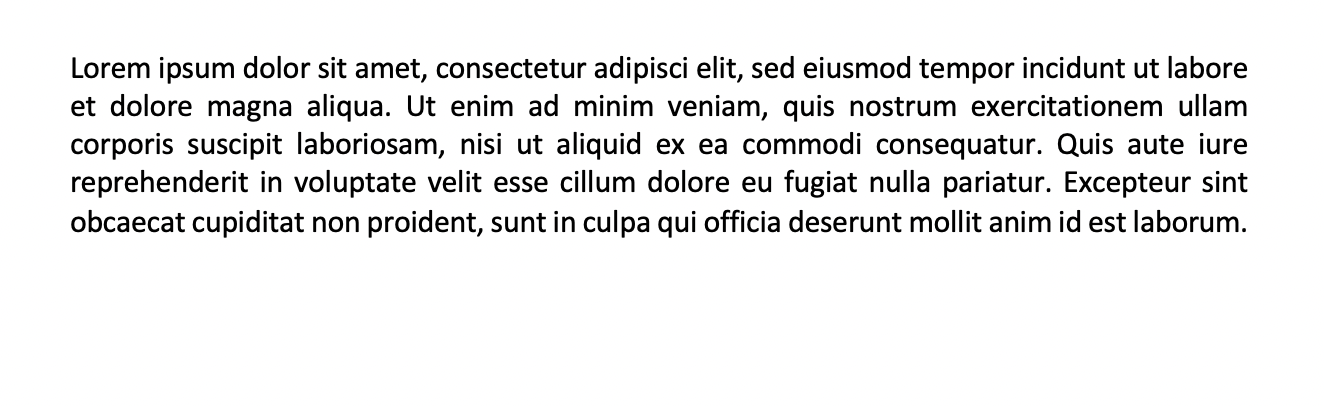
\includegraphics[width=8cm, height=10cm, keepaspectratio]{lorem.png}}
        \caption{Allegato poesia.doc}\label{allegatoWord}
      \end{figure}



    \pagebreak
    \subsection{Test sull'analisi del contesto}
    


\begin{table}[htp]
    \vspace{4.5cm}
    \centering
    \resizebox{\textwidth}{!}{%
    \begin{tabular}{ll}
    \multicolumn{2}{c}{test 7 (TS07): \textbf{Messaggio indirizzato al dominio topolino.it}}                                                       \\ \hline
    \rowcolor[HTML]{EFEFEF} 
    \multicolumn{1}{|l|}{\cellcolor[HTML]{EFEFEF}ID}    & \multicolumn{1}{l|}{\cellcolor[HTML]{EFEFEF}TS07}                            \\ \hline
    \multicolumn{1}{|l|}{Nome}                          & \multicolumn{1}{l|}{Messaggio indirizzato al dominio topolino.it}               \\ \hline
    \rowcolor[HTML]{EFEFEF} 
    \multicolumn{1}{|l|}{\cellcolor[HTML]{EFEFEF}Descrizione} &
      \multicolumn{1}{l|}{\cellcolor[HTML]{EFEFEF}\begin{tabular}[c]{@{}l@{}}il messaggio è stato inviato ad un \\ dominio bloccato da policy.\end{tabular}} \\ \hline
    \multicolumn{1}{|l|}{\begin{tabular}[c]{@{}l@{}}Messaggio inviato\\ dal mittente\end{tabular}} &
      \multicolumn{1}{l|}{\begin{tabular}[c]{@{}l@{}}Subject: test invio\\ From: Paolo Fagioli <paolo.fagioli@certimeter.it>\\ To: Paolo Fagioli <p.fagioli@topolino.it>\\ \\ prova\end{tabular}} \\ \hline
    \rowcolor[HTML]{EFEFEF} 
    \multicolumn{1}{|l|}{\cellcolor[HTML]{EFEFEF}Risultato atteso} &
      \multicolumn{1}{l|}{\cellcolor[HTML]{EFEFEF}\begin{tabular}[c]{@{}l@{}}Verrà attivata la clausola REJECT, il messaggio\\ sarà rifiutato da Postfix e verrà avvisato il\\ mittente.\end{tabular}} \\ \hline
    \multicolumn{1}{|l|}{Risultato ottenuto} &
      \multicolumn{1}{l|}{\begin{tabular}[c]{@{}l@{}}Postfix ha rifiutato il messaggio. Il mittente ha\\ ricevuto il seguente avviso:\\ \\ RECIPIENT DOMAIN BANNED\end{tabular}} \\ \hline
    \rowcolor[HTML]{EFEFEF} 
    \multicolumn{1}{|l|}{\cellcolor[HTML]{EFEFEF}Esito} & \multicolumn{1}{l|}{\cellcolor[HTML]{EFEFEF}{\color[HTML]{333333} SUPERATO}} \\ \hline
    \end{tabular}%
    }
    \end{table}


\begin{table}[htp]
    \centering
    \resizebox{\textwidth}{!}{%
    \begin{tabular}{ll}
    \multicolumn{2}{c}{test 8 (TS08): \textbf{Messaggio inviato da mittente in blacklist}} \\ \hline
    \rowcolor[HTML]{EFEFEF} 
    \multicolumn{1}{|l|}{\cellcolor[HTML]{EFEFEF}ID} &
      \multicolumn{1}{l|}{\cellcolor[HTML]{EFEFEF}TS08} \\ \hline
    \multicolumn{1}{|l|}{Nome} &
      \multicolumn{1}{l|}{Messaggio inviato da mittente in blacklist} \\ \hline
    \rowcolor[HTML]{EFEFEF} 
    \multicolumn{1}{|l|}{\cellcolor[HTML]{EFEFEF}Descrizione} &
      \multicolumn{1}{l|}{\cellcolor[HTML]{EFEFEF}\begin{tabular}[c]{@{}l@{}}il messaggio è stato inviato da un \\ mittente che si trova in blacklist.\end{tabular}} \\ \hline
    \multicolumn{1}{|l|}{\begin{tabular}[c]{@{}l@{}}Messaggio inviato\\ dal mittente\end{tabular}} &
      \multicolumn{1}{l|}{\begin{tabular}[c]{@{}l@{}}Subject: avviso\\ From: Francesco Lorusso <francesco.lorusso@certimeter.it>\\ To: Paolo Fagioli <paolo.fagioli@certimeter.it>\\ \\ ciao Paolo,\\ ti avviso che domani non sarà possibile vederci.\end{tabular}} \\ \hline
    \rowcolor[HTML]{EFEFEF} 
    \multicolumn{1}{|l|}{\cellcolor[HTML]{EFEFEF}Risultato atteso} &
      \multicolumn{1}{l|}{\cellcolor[HTML]{EFEFEF}\begin{tabular}[c]{@{}l@{}}Verrà attivata la clausola REJECT, il messaggio\\ sarà rifiutato da Postfix e verrà avvisato il\\ mittente.\end{tabular}} \\ \hline
    \multicolumn{1}{|l|}{Risultato ottenuto} &
      \multicolumn{1}{l|}{\begin{tabular}[c]{@{}l@{}}Postfix ha rifiutato il messaggio. Il mittente ha\\ ricevuto il seguente avviso:\\ \\ SENDER ADDRESS REJECTED: BLACKLISTED\end{tabular}} \\ \hline
    \rowcolor[HTML]{EFEFEF} 
    \multicolumn{1}{|l|}{\cellcolor[HTML]{EFEFEF}Esito} &
      \multicolumn{1}{l|}{\cellcolor[HTML]{EFEFEF}{\color[HTML]{333333} SUPERATO}} \\ \hline
    \end{tabular}%
    }
    \end{table}




